% Created 2020-07-22 Wed 18:17
% Intended LaTeX compiler: pdflatex
\documentclass[11pt]{article}
\usepackage[utf8]{inputenc}
\usepackage[T1]{fontenc}
\usepackage{graphicx}
\usepackage{grffile}
\usepackage{longtable}
\usepackage{wrapfig}
\usepackage{rotating}
\usepackage[normalem]{ulem}
\usepackage{amsmath}
\usepackage{textcomp}
\usepackage{amssymb}
\usepackage{capt-of}
\usepackage{hyperref}
\author{Mike Chyson}
\date{\today}
\title{}
\hypersetup{
 pdfauthor={Mike Chyson},
 pdftitle={},
 pdfkeywords={},
 pdfsubject={},
 pdfcreator={Emacs 26.3 (Org mode 9.1.9)}, 
 pdflang={English}}
\begin{document}

\tableofcontents

\section{Autoencoders}
\label{sec:orgf2e8d7e}
An \textbf{autoencoder} is a neural network that is trained to attempt to copy its input to its output. Internally, it has a hidden layer \(h\) that describes a \textbf{code} used to represent the input. The network may be viewed as consisting of two parts: an encoder function \(h=f(x)\) and a decoder that produces a reconstruction \(r=g(h)\). This architecture is presented in Fig. 14.1.\\

\begin{center}
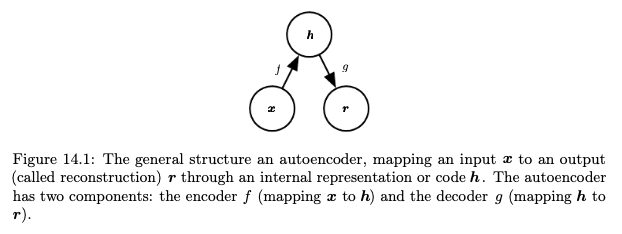
\includegraphics[width=.9\linewidth]{pics/figure14.1-autoencoder.png}
\end{center}

If an autoencoder succeeds in simply learning to set \(g(f(x)) = x\) everywhere, then it is not especially useful. Instead, autoencoders are \textbf{designed to be unable to learn to copy perfectly}. Usually they are restricted in ways that allow them to \textbf{copy only approximately, and to copy only input that resembles the training data}. Because the model is forced to prioritize which aspects of the input should be copied, it often learns useful properties of the data.\\


Modern autoencoders have generalized the idea of an encoder and a decoder beyond deterministic functions to stochastic mappings \(p_{encoder}(h | x)\) and \(p_{decoder}(x | h)\).\\

Traditionally, autoencoders were used for dimensionality reduction or feature learning. Recently, \textbf{theoretical connections between autoencoders and latent variable models} have brought autoencoders to the forefront of generative modeling.\\

\subsection{Undercomplete Autoencoders}
\label{sec:org4d69cc3}
Copying the input to the output may sound useless, but we are typically not interested in the output of the decoder. Instead, we hope that training the autoencoder to perform the input copying task will result in \(h\) taking on \textbf{useful properties}.\\

One way to obtain useful features from the autoencoder is to constrain \(h\) to have smaller dimension than \(x\). An autoencoder whose code dimension is less than the input dimension is called \textbf{undercomplete}. Learning an undercomplete representation forces the autoencoder to capture the \textbf{most salient features} of the training data.\\


The learning process is described simply as minimizing a loss function\\
\begin{equation}
L(x,g(f(x)))
\end{equation}
Where \(L\) is a loss function penalizing \(g(f(x))\) for being dissimilar from \(x\), such as the mean squared error.\\


When the decoder is linear and \(L\) is the mean squared error, an undercomplete autoencoder learns to span the same subspace as PCA. In this case, an autoencoder trained to perform the copying task has learned the principal subspace of the training data as a side-effect.\\


Autoencoders with nonlinear encoder functions \(f\) and nonlinear decoder functions \(g\) can thus learn a more powerful nonlinear generalization of PCA. \textbf{Unfortunately, if the encoder and decoder are allowed too much capacity, the autoencoder can learn to perform the copying task without extracting useful information about the distribution of the data.}\\


An autoencoder trained to perform the copying task can fail to learn anything useful about the dataset if the capacity of the autoencoder is allowed to become too great.\\



\subsection{Regularized Autoencoders}
\label{sec:org4f4ff14}
Undercomplete autoencoders, with code dimension less than the input dimension, can learn the most salient features of the data distribution. Autoencoders fail to learn anything useful if the encoder and decoder are given too much capacity (unlinear method).\\

A similar problem occurs if the hidden code is allowed to have dimension equal to the input, and in the \textbf{overcomplete} case in which the hidden code has dimension greater than the input. In these cases, even a \textbf{linear} encoder and \textbf{linear} decoder can learn to copy the input to the output without learning anything useful about the data distribution.\\



Ideally, one could train any architecture of autoencoder successfully, choosing the code dimension and the capacity of the encoder and decoder based on the complexity of distribution to be modeled. Regularized autoencoders provide the ability to do so.\\


Rather than limiting the model capacity by keeping the encoder and decoder shallow and the code size small, regularized autoencoders use a \textbf{loss function} that encourages the model to have \textbf{other properties} besides the ability to copy its input to its output. These other properties include:\\
\begin{itemize}
\item sparsity of the representation,\\
\item smallness of the derivative of the representation, and\\
\item robustness to noise or\\
\item to missing inputs.\\
\end{itemize}
A regularized autoencoder can be nonlinear and overcomplete but still learn something useful about the data distribution even if the model capacity is great enough to learn a trivial identity function.\\

In addition to the methods described here which are most naturally interpreted as regularized autoencoders, \textbf{nearly any generative model with latent variables and equipped with an inference procedure} (for computing latent representations given input) may be viewed as a particular form of \textbf{autoencoder}.\\


\subsubsection{Sparse Autoencoders}
\label{sec:org784f96f}
A spare autoencoder is simply an autoencoder whose training criterion involves a sparsity penalty \(\Omega(h)\) on the code layer \(h\), in addition to the reconstruction error:\\
\begin{equation}
L(x,g(f(x))) + \Omega(h)
\end{equation}
where \(g(h)\) is the decoder output and typically we have \(h=f(x)\), the encoder output.\\

\textbf{Sparse autoencoders are typically used to learn features for another task such as classification.} An autoencoder that has been regularized to be sparse must respond to unique statistical features of the dataset it has been trained on, rather than simply acting as an identity function. In this way, training to perform the copying task with a sparsity penalty can yield a model that has learned useful features as a \textbf{byproduct}.\\


We can think of the penalty \(\Omega(h)\) simply as a regularizer term added to a feedforward network whose primary task is to copy the input to the output (unsupervised learning objective) and possibly also perform some supervised task (with a supervised learning objective) that depends on these sparse features. Unlike other regularizers such as weight decay, there is not a straightforward Bayesian interpretation to this regularizer. We can still think of these regularization terms as implicitly expressing a preference over functions.\\


Rather than thinking of the sparsity penalty as a regularizer for the copying task, we can think of the entire sparse autoencoder framework as approximating maximum likelihood training of a generative model that has latent variables.\\


Suppose we have a model with visible variables \(x\) and latent variables \(h\), with explicit joint distribuction \(p_{model}(x,h) = p_{model}(h)p_{model}(x|h)\). We refer to \(p_{model}(h)\) as the model's prior distribution over t he latent varaibles, representing the model's beliefs prior to seeing \(x\). The log-likelihood can be decomposed as\\
\begin{equation}
\log p_{model}(x) = \log \sum_h p_{model}(h,x).
\end{equation}

We can think of the autoencoder as approximating this sum with a point estimate for just one highly likely value for \(h\). From this point of view, with this chosen \(h\), we are maximizing\\
\begin{equation}
\log p_{model}(h,x) = \log p_{model}(h) + \log p_{model}(x|h).
\end{equation}


The \(\log p_{model}(h)\) term can be sparsity-inducing.\\
For example, the Laplace prior,\\
\begin{equation}
p_{model}(h_i) = \frac{\lambda}{2} e^{-\lambda|h_i|},
\end{equation}
corresponds to an absolute value sparsity penalty. Expressing the log-prior as an absolute value penalty, we obtain\\
\begin{equation}
\Omega(h) = \lambda \sum_i |h_i|
\end{equation}
\begin{equation}
-\log p_{model}(h) = \sum_i(\lambda|h_i| - \log\frac{\lambda}{2}) = \Omega(h) + \mathrm{const}
\end{equation}
where the constant term depends only on \(\lambda\) and not \(h\). We typically treat \(\lambda\) as a hyperparameter and discard the constant term since it does not affect the parameter learning. Other priors such as the Student-t prior can also induce sparsity.\\

From this point of view of sparsity as resulting from the effect of \(p_{model}(h)\) on approximate maximum likelihood learning, the sparsity penalty is not a regularization term at all. It is just a consequence of the \textbf{model’s distribution over its latent variables}. It provides a different reason for why the features learned by the autoencoder are useful: they describe the \textbf{latent variables} that explain the input.\\


One way to achieve \textbf{actual zeros} in \(h\) for sparse (and denoising) autoencoders was introduced in Glorot et al. (2011b). The idea is to use \textbf{rectified linear units} to produce the code layer.\\


\subsubsection{Denoising Autoencoders}
\label{sec:org7e8cec5}
Rather than adding a penalty \(\Omega\) to the cost function, we can obtain an autoencoder that learns something useful by changing the reconstruction error term of the cost function.\\


A \textbf{denoising autoencoder} or DAE minimizes\\
\begin{equation}
L(x,g(f(\tilde{x}))),
\end{equation}
where \(\tilde{x}\) is a copy of \(x\) that has been corrupted by some form of noise. Denoising autoencoders must therefore undo this corruption rather than simply copying their input.\\



Denoising training forces \(f\) and \(g\) to implicitly learn the structure of \(p_{data}(x)\). Denoising autoencoders thus provides yet another example of how \textbf{useful properties} can emerge as a \textbf{byproduct} of minimizing reconsutrction error. They are also an example of how overcomplete, high-capacity models may be used as autoencoders so long as care is taken to prevent them from learning the identity function.\\


\subsubsection{Regularizing by Penalizing Derivatives}
\label{sec:org7d98ca5}
Another strategy for regularizing an autoencoder is to use a penalty \(\Omega\) as in sparse autoencoders,\\
\begin{equation}
L(x,g(f(x))) + \Omega(h,x),
\end{equation}
but with a different form of \(\Omega\):\\
\begin{equation}
\Omega(h,x) = \lambda \sum_i ||\nabla_x h_i||^2.
\end{equation}
This forces the model to learn a function that does not change much when \(x\) changes slightly. Because this penalty is applied only at training examples, it forces the autoencoder to learn features that capture information about the training distribution.\\


An autoencoder regularized in this way is called a \textbf{contractive autoencoder} or CAE. This approach has theoretical connections to denoising autoencoders, manifold learning and probabilistic modeling.\\


\subsection{Representation Power, Layer Size and Depth}
\label{sec:org5ab1de7}
Autoencoders are \textbf{often} trained with only a \textbf{single layer encoder} and a \textbf{single layer decoder}. However, this is \textbf{not a requirement}. In fact, using deep encoders and decoders offers many advantages.\\


There are many advantages to depth in a feedforward network. Because autoencoders are feedforward networks, these advantages also apply to autoencoders. Moreover, the encoder is itself a feedforward network as is the decoder, so each of these components of the autoencoder can individually benefit from depth.\\


One major advantage of non-trivial depth is that the \textbf{universal approximator theorem} guarantees that a \textbf{feedforward neural network with at least one hidden layer can represent an approximation of any function (within a broad class) to an arbitrary degree of accuracy, provided that it has enough hidden units.} This means that an autoencoder with a single hidden layer is able to represent the identity function along the domain of the data arbitrarily well. However, the mapping from input to code is shallow. This means that we are not able to enforce arbitrary constraints, such as that the code should be sparse. A deep autoencoder, with at least one additional hidden layer inside the encoder itself, can approximate any mapping from input to code arbitrarily well, given enough hidden units.\\

Depth can exponentially reduce the computational cost of representing some functions. Depth can also exponentially decrease the amount of training data needed to learn some functions.\\

Experimentally, deep autoencoders yield much better compression than corresponding shallow or linear autoencoders (Hinton and Salakhutdinov, 2006).\\

A common strategy for training a deep autoencoder is to \textbf{greedily pretrain} the deep architecture by training a stack of shallow autoencoders, so we often encounter shallow autoencoders, even when the ultimate goal is to train a deep autoencoder.\\



\subsection{Stochastic Encoders and Decoders}
\label{sec:org7aa9d84}
Autoencoder are just feedforward networks.\\


In an autoencoder, \(x\) is now the target as well as the input. Yet we can still apply the same machinery as in feedforward.\\

Given a hidden code \(h\), we may think of the decoder as providing a conditional distribution \(p_{decoder}(x | h)\). We may then train the autoencoder by minimizing \(−\log p_{decoder}(x | h)\). The exact form of this loss function will change depending on the form of \(p_{decoder}\) . As with traditional feedforward networks, we usually use linear output units to parametrize the mean of a Gaussian distribution if \(x\) is real-valued. In that case, the negative log-likelihood yields a mean squared error criterion. Similarly, binary \(x\) values correspond to a Bernoulli distribution whose parameters are given by a sigmoid output unit, discrete \(x\) values correspond to a softmax distribution, and so on.\\


To make a more radical departure from the feedforward networks we have seen previously, we can also generalize the notion of an \textbf{encoding function} \(f(x)\) to an encoding distribution \(p_{encoder}(h | x)\), as illustrated in Fig. 14.2.\\

\begin{center}
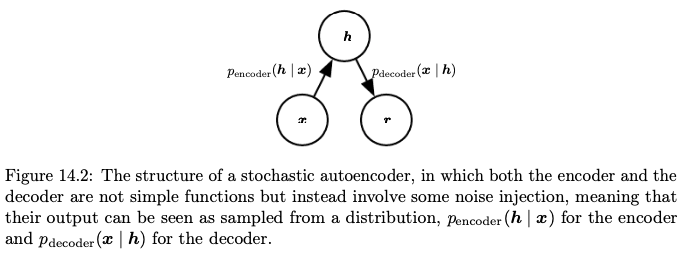
\includegraphics[width=.9\linewidth]{pics/figure14.2-stochastic-autoencoder.png}
\end{center}


Any latent variable model \(p_{model}(h,x)\) defines a stochastic encoder\\
\begin{equation}
p_{encoder}(h|x) = p_{model}(h|x)
\end{equation}
and a stochastic decoder\\
\begin{equation}
p_{decoder}(x|h) = p_{model}(x|h).
\end{equation}
In general, the encoder and decoder distributions are not necessarily conditional distributions compatible with a unique joint distribution \(p_{model}(x, h)\).\\


Alain et al. (2015) showed that training the encoder and decoder as a denoising autoencoder will tend to make them compatible asymptotically (with enough capacity and examples).\\


\subsection{Denoising Autoencoders}
\label{sec:org3034bc8}
The denoising autoencoder (DAE) is an autoencoder that receives a corrupted data point as input and is trained to predict the original, uncorrupted data point as its output.\\

The DAE training procedure is illustrated in Fig. 14.3.\\

\begin{center}
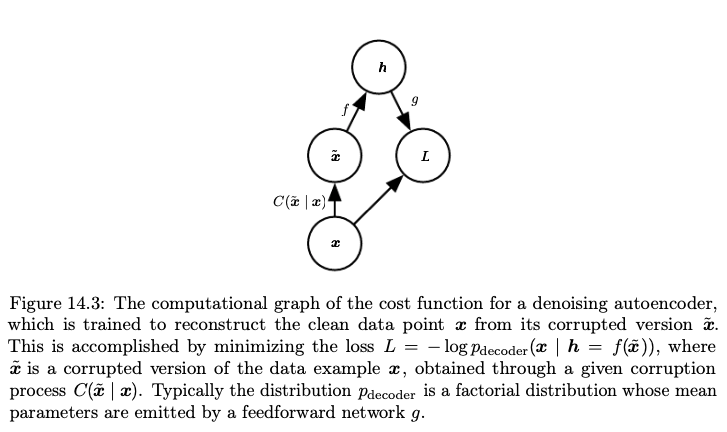
\includegraphics[width=.9\linewidth]{pics/figure14.3-denoising-autoencoder.png}
\end{center}

\(C(\tilde{\mathbf{x}}|\mathbf{x})\) represents a conditional distribution over corrupted samples \(\tilde{\mathbf{x}}\), given a data sample \(\mathbf{x}\). The autoencodet learns a \textbf{reconstruction distribution} \(p_{reconstruct}(\mathbf{x}|\tilde{\mathbf{x}})\) estimated from training pairs \((x,\tilde{x})\), as follows:\\
\begin{enumerate}
\item Sample a training example \(x\) from the training data.\\
\item Sample a corrupted version \(\tilde{x}\) from \(C(\tilde{\mathbf{x}}|\mathbf{x}=x)\)\\
\item Use \((x,\tilde{x})\) as a training example for estimating the autoencoer reconstruction distribution \(p_{reconstruct}(x|\tilde{x})=p_{decoder}(x|h)\) with \(h\) output of encoder \(f(\tilde{x})\) and \(p_{decoder}\) typically defined by a decoder \(g(h)\)\\
\end{enumerate}


Typically we can simply perform gradient-based approximate minimization (such as minibatch gradient descent) on the negative log-likelihood \(− \log p_{decoder}(x | h)\).\\


We can threrefore view the DAE as performing stochastic gradient descent on the following expectation:\\
\begin{equation}
-\mathbb{E}_{\mathbf{x}~\hat{p}_{data}(\mathbf{x})} \mathbb{E}_{\tilde{\mathbf{x}}~C(\tilde{mathbf{x}}|x)} \log p_{decoder}(x|h=f(\tilde{x})),
\end{equation}
where \(\tilde{p}(x)\) is the training distribution.\\


\subsubsection{Estimating the Score}
\label{sec:orgefa46a2}
\textbf{Score matching} (Hyvärinen, 2005) is an \textbf{alternative to maximum likelihood}. It provides a consistent estimator of probability distributions based on encouraging the model to have the same score as the data distribution at every training point \(x\). In this context, the score is a particular gradient field:\\
\begin{equation}
\nabla_x \log p(x).
\end{equation}

Learning the gradient field of \(\log p_{data}\) is one way to learn the structure of \(p_{data}\) itself.\\


A very important property of DAEs is that their training criterion (with conditionally Gaussian \(p(|h)\)) makes the autoencoder learn a vector field \((g(f(x)) − x)\) that estimates the score of the data distribution. This is illustrated in Fig. 14.4.\\

\begin{center}
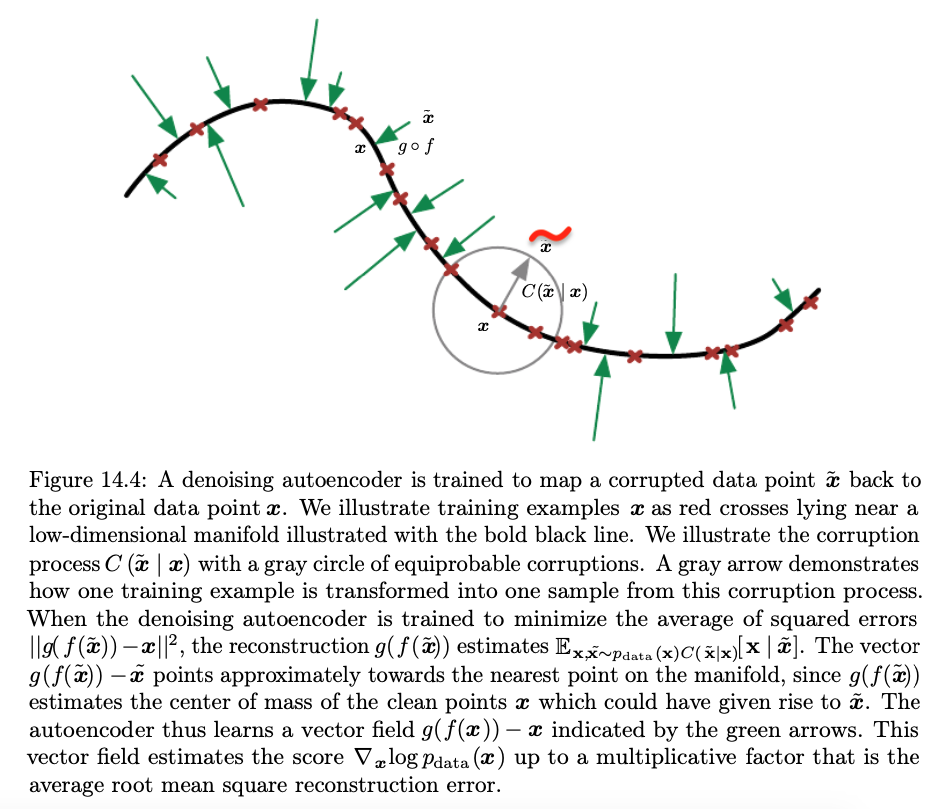
\includegraphics[width=.9\linewidth]{pics/figure14.4-score-matching.png}
\end{center}

Denoising training of a specific kind of autoencoder (sigmoidal hidden units, linear reconstruction units) using Gaussian noise and mean square error as the reconstruction cost is equivalent (Vincent, 2011) to training a specific kind of undirected probabilistic model called an RBM with Gaussian visible units. RBM is a model that provides an explicit \(p_{model}(x;\theta)\). When the RBM is trained using denoising score matching (Kingma and LeCun, 2010), its learning algorithm is equivalent to denoising training in the corresponding autoencoder.\\

With a fixed noise level, regularized score matching is not a consistent estimator; it instead recovers a blurred version of the distribution. However, if the noise level is chosen to approach 0 when the number of examples approaches infinity, then consistency is recovered.\\


Score matching applied to RBMs yields a cost function that is identical to reconstruction error combined with a regularization term similar to the contractive penalty of the CAE (Swersky et al., 2011). Bengio and Delalleau (2009) showed that an autoencoder gradient provides an approximation to contrastive divergence training of RBMs.\\


For continuous-valued \(x\), the denoising criterion with Gaussian corruption and reconstruction distribution yields an estimator of the score that is applicable to general encoder and decoder parametrizations (Alain and Bengio, 2013). This means a generic encoder-decoder architecture may be made to estimate the score by training with the squared error criterion\\
\begin{equation}
||g(f(\tilde{x}) - x||^2
\end{equation}
and corruption\\
\begin{equation}
C(\tilde{\mathbf{x}} = \tilde{x}|x) = \mathcal{N}(\tilde{x}; \mu = x, \Sigma = \sigma^2 I)
\end{equation}
with noise variance \(\sigma^2\)\\


In general, there is no guarantee that the reconstruction g(f (x)) minus the input x corresponds to the gradient of any function, let alone to the score.\\

\subsubsection{Historical Perspective}
\label{sec:org23d3177}
The idea of using MLPs for denoising dates back to the work of LeCun (1987) and Gallinari et al. (1987). Behnke (2001) also used recurrent networks to denoise images. Denoising autoencoders are, in some sense, just MLPs trained to denoise. However, the name "denoising autoencoder" refers to a model that is intended not merely to learn to denoise its input but to learn a good internal representation as a side effect of learning to denoise.\\


Like sparse autoencoders, sparse coding, contractive autoencoders and other regularized autoencoders, the motivation for DAEs was to allow the learning of a very high-capacity encoder while preventing the encoder and decoder from learning a useless identity function.\\
\end{document}